As mentioned in the introduction, the goal is to create sets of registrations that can be seen as families. This is done in three phases: the matching of individual registrations based on the names of the persons that are mentioned on the registrations. The second phase is to check these matches for complience on extra constraints on the names and on the distance between the names and to filter out the matches with an undesired distance. In the third phase, we will filter out the matches that do not comply with the extra constraints on internal consistency. \newline

The first step will create a set of matches between the candidate sets, one for each type of registration, and the target set. For each target entry, the matched candidate entries can be seen as a family: these candidate entries are the registrations for which the names of both the parents are similar to the target entry, within a allowed error over all the names. Matches in this step will be made using the Levenshtein distance. The distance is calculated over the entire string of all four names. For a detailed description of the Levenshtein distance, see appendix A. We assume that all the candidate entries that are matched to the same target entry are registrations of life events of childern that have the same parents, as the names of the candidate entries are the names of the \textit{parents} for the person that the registration was made for. These names are matched to the same names of a target entry: the names of the groom and  bride on a marriage certificate. In order to generate overlinking, the matching is done with an allowed distance of 3, 4 and 5 over the entire string of names.\\

In the second step, the results from the first step are checked for complience on extra constraints in order to filter out those matches that are accepted in the first step where the (allowed) error is too much concentrated in a single name. In the first step, we calculated the edit distance over the entire string of all names, and accepted a match when the distance did not exceed the threshold. This means that the entire allowed error could be concentrated in a single name. This could be acceptable, given that the length of the name is sufficient to justify such an error, but it might also mean that the names differ completely when the names are shorter, or of equal length to the allowed error. The second step will introduce rules to rule out such unwanted matches.\newline

The third step is to check if the resulting sets of families of the second step are consistent with a set of constrains, filtering out those that are not. The set of constraints are based on knowledge about the real world. For instance: it is impossible for a person to be born after his/her mother has passed away. These (simple) rules will filter out matches that have slipped past the checks in both step one and two. \newline

The accuracy of the matching in the first phase will have a large impact on the size of the families. Since matching in the first phase is done on the Levenshtein distance, the maximum allowed distance will determine the extend to which overlinking (or underlinking, if the allowed distance is too strict) will occur. From a computational point of view, the first step should be as close to the real situation as possible. However, allowing overlinking in this step might not be considered a bad choice. Since the results in the first phase will be filtered in the second phase, the degree of overlinking will be smaller after the filtering in the second step. Another consideration is that underlinking could result in true matches being missed. Matches that have been missed in the first step can not be retrieved in the later steps of the process. \newline

Ideally, a family will include the birth certificates, marriage and death certificates of all the children. However, this will not always be the case. For instance, problems with matching will arise when trying to match death certificates to the target entries. For some of the death certificate registrations, the parents are not mentioned on the death certificate and there are other cases where the father or mother has remarried. 
In the latter case the new partner of the father is mentioned on the certificate in stead of the mother of the person who has died, creating a new pair of parents, or no second parent is mentioned. This obviously will pose a problem when matching against the target entries. In case one of the parents has remarried, another entry with the names of the new parent pair will also be present in the target set (as the new marriage will have it's own marriage registration). This will lead to a mismatch: the birth certificate will be matched to the correct pair of parents, whereas the death certificate will be  matched to the second pair of parents, or, in the case that one of the parents are missing, will not be matched at all since the error is too large.  \newline

Another possiblity is that the same certificate will be matched to two different pairs of parents when the names of both pairs of parents are identical. When two set of parents have exact matching names, the same certificate will be added to both the families of these pairs. Since it was common practice that children were named after members of their family, the chances of identical names for the four parents are not negligible. However, since there are 4 different persons involved there is still a small chance that this occurs. We will refer to the fact that a single certificate is matched to more than one parent pair as overlinking.\newline

\section{String matching}
In the first step, the matching is done by using the approach as described in \cite{Aspects001}. This approach is used to create the set of families in an efficient way, in order to avoid matching all the candidate registrations to each of the target registrations. The approach uses a tree sorting algorithm to filter out the registrations that, given some maximum Levenshtein distance, are not to be considered as a match and mapping the target registrations to the candidate registrations that are considered as viable matches. The registrations that are left after filtering are compared to the target registration using the Levenshtein distance. \\
The target registrations are used to build the tree. For each candidate registration, a tree traversal is done. All the target registrations of the vectors in leaf nodes that can be reached with a certain edit distance are considered a potential match for the candidate registration. As a result from the tree traversal, each candidate registration is mapped to one or more target registrations, and each target registration has a set of candidate registrations. Two registrations are considered a match when the Levenshtein distance is below the predefined threshold. \\
The approach is to use the registrations of the children (that is: birth, marriage and death certificates) as the \textit{candidate} certificates, and the certificates of the marriages of the parents as the \textit{target} certificates.

\subsection{Building the vectortree}

Each name on the target registrations will be transformed into a bit vector of eight bits. Each position in the bit vector represents a set of letters, as shown in table \ref{tab:letterpositions}. For each position in the bit vector, the letters corresponding to that position will be searched in the name. If at least one of those letters is found in the name, the position in the bit vector will be true, otherwise that position will be false.  \\

\begin{table}
	\centering
	\caption[Position of letters in a bitvector]{\label{tab:letterpositions}The positions in the bit vector represent certain letters. For each name, eight positions are available and if a letter occurs in the name, the corresponding bit is `activated'. For example: using the sets of letters in table \ref{tab:letterpositions} the name \textit{Jobse} will be converted to the vector $\langle1,1,0,0,0,0,1,1\rangle$}
	\vspace{0.5cm}
	\begin{tabular}{lc}
		\toprule
		letters & position \\
		\midrule
		$\{e, g\}$ & 0\\
		$\{a,l,q,h,j,x,comma\}$ & 1\\
		$\{r,p,v\}$ & 2\\
		$\{n, space\}$ & 3\\
		$\{i, u, w\}$ & 4\\
		$\{d,f,c,m,z\}$ & 5\\
		$\{t,s,y\}$ & 6\\
		$\{o,b,k,other\}$ & 7\\
		\bottomrule
	\end{tabular}
	
	
\end{table}
In the case of the target registrations, the resulting bit vector will be used to build the vectortree. The tree starts with a single node, representing the first position in the bit vector. Nodes and edges are added when iterating over the bit vector, by checking for each position in the bitvector if there is an edge from the previous node corresponding with the previous position in the bitvector to a node that correspond to the value of the current position. 
If this is not the case, a new child node and edge are inserted in the tree. If such edge and node exists, this edge is followed and the next position is evaluated. When the last position of the bit vector is evaluated, the certificate is added to the leave node. This leaf node contains all the certificates with the same bit vector, generating a set of potential target certificates for a candidate certificate. \\

In order to make this procedure more clear, consider the following example. We are building a vectortree for words that consists of the alphabet ${a, b, c}$, and the bit vectors are of length 3, encoding occurrences of these three letters. The word $aaa$ will therefore be converted to $\langle 1,0,0 \rangle$ and the word $abc$ will be converted to $\langle 1,1,1 \rangle$. \\
In figure \ref{fig:partial_vectree} a partial tree is shown. We would like to add the word $abbab$ to the tree. The bit vector will be $\langle1,1,0\rangle$. Since the first position in the bit vector has a value of 1, the edge with label 1 will be taken in the first node. The same holds for the second position. However, for the third position a new edge and node will be added to the three, since none of the previous words have created this edge.

\begin{figure}
	\begin{center}
		\caption[A partial vectortree]{A (partial) vectortree when build on words from the alphabet $a,b,c$. Adding the word $abbab$ will add the dotted edge and node to the tree. \label{fig:partial_vectree}}
		\vspace{0.5cm}
	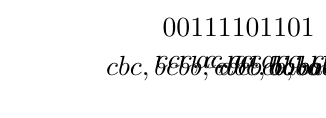
\begin{tikzpicture}[every tree node/.style={draw,circle},
	level distance=1.25cm,sibling distance=1cm,
	edge from parent path={(\tikzparentnode) -- (\tikzchildnode)}]
	\Tree 
	[.a 
		\edge node[midway,left] {$0$};
		[.b
			\edge node[midway,left] {$0$};
			[.c
				\edge node[auto=right] {$1$};
				[.\node [label=below:${ccc,c,cc}$] {}; ]
			]
			\edge node[midway,right] {$1$};
			[.c
				\edge node[auto=right] {$1$};
				[.\node [label=below:${cbc,bcbb,cbcbcb,bbbbc}$] {}; ] 
			]
		]
		\edge node[midway,right] {$1$};
		[.b
			\edge node[midway,left] {$0$};
			[.c
				\edge node[auto=right] {$1$};
				[.\node [label=below:${ac, acacc, cca}$] {}; ]
			]
			\edge node[midway,right] {$1$};
			[.c
				\edge [dotted] node[auto=right] {$0$};
				[.\node [dotted,label=below:${abbab}$] {}; ]
				\edge node[auto=right] {$1$};
				[.\node [label=below:${abc, bacacc, cbca}$] {}; ]
			]
		]	
	]
	\end{tikzpicture}
	

			
\end{center}
\end{figure}

\subsection{Matching the candidates}
The bit vectors of the candidate set are matched by traversing the vectortree, based on the values of the bit vector generated for that candidate. If a path to a leaf node exists, all the target registrations in the leaf node are considered a match, and if no such leaf node can be reached, the candidate is discarded. Tree-traversal is done by exploring all the possible branches in the tree, but a branch is pruned if the difference between the current path and path corresponding to the bit vector (that is, all the paths which labels correspond to the values of the bits in the bit vector) exceeds some predefined threshold.  
\newline

Since the matches are based on the values of the bit vectors, the strings of the matches do not necessarily need to be exactly the same. Therefore, the Levenshtein distance is used to calculate the exact distance. However, since the bit vector groups certain letters into a single group, potential matches that are within the Levenshtein distance could be missed when only taking the leaf node on the direct path into account. 
For example, when matches with an edit distance of 1, the legitimate match between the names \textit{Zegers} and \textit{Segers} will not be in the same leaf node and therefore are not considered to be a match when only taking the matches into account that are in the same leaf node. For example: the bitvector of the names \textit{Zegers} and \textit{Segers} are $\langle 1, 0, 1, 0, 0, 1, 0, 0\rangle$ and $\langle 1, 0, 1, 0, 0, 0, 1, 0\rangle$, respectively. Upto bit 5, these vectors are completely the same, and therefore follow the same path.
\newline

In order to compensate for this, the paths that are accessible within the maximum error are also considered, and the registrations in the corresponding leaf nodes are added to the set of potential matches.

\section{Matching with higher thresholds}
\subsection{Name pair matching}
\label{sec:name_pair_matching}
In the method described above, the edit distance is calculated over the strings of all four names. This could lead to false negatives: the maximum edit distance is exceeded and the match is rejected, but the match should have been accepted. There are many names in the Dutch language that have alternative writing styles. Examples are first names like \textit{Cornelis} / \textit{Kornelis} and \textit{Lourens} / \textit{Laurens} or surnames like \textit{Huizen} / \textit{Huijzen} or \textit{Belsen} / \textit{Belzen}. 
The similarity between these name variants is that the variants share the same semi-phonetic form, although the spelling is different. This adds at least a cost of 1 to the (levenshtein) edit distance, where there is a good reason to ignore these kinds of name variants. 



% Voorbeeld toevoegen
In \cite{bloothooft2014learning} a set of decision rules was proposed to accept matches based on the edit distance per name. Matching was done not only based on edit distance, but also on the additional constraint that matches must share the same prefix. This was done in order to accept matches for name pairs with higher Levenshtein distances. The constraint on the length of the shared prefix is determined by the edit distance between the two matches, as shown in table \ref{tab:Ruleset}. The constraint on the length demands that, for a given length, either the shortest or the longest name in the name pair is of a certain length (depending on the length of the distance), and the constraint on the prefix demands that both names start with the same sequence of characters. There is also an additional rule, demanding that if the the length of the concatenation of both names minus the edit distance is greater than 16 and the names start with the same letter, the match is also accepted.

\begin{table}
	\centering
	\caption[Extra rules for name based matching]{\label{tab:Ruleset} The set of extra rules when matching is done on single names. The rules are more strict when the Levenshtein distance increases. }
	\vspace{0.5cm}
	\begin{tabular}{ccc}
		\toprule
		Levenshtein distance & length & length matching prefix \\
		\midrule
		1 & shortest $>$ 4 & 1 \\
		2 & shortest $>$ 4 & 2 \\
		3 & longest $>$ 5 & 3 \\
		4 & longest $>$ 7 & 4 \\
		5 & longest $>$ 8 & 4 \\
		\midrule
		\multicolumn{2}{c}{total length of pair minus Levenshtein distance $>$ 16} & 1 \\
		\bottomrule
	\end{tabular}
\end{table}

\subsection{Allowing more distance}
Although \cite{bloothooft2014learning} applied these rules to name pairs for which the names have been converted into semi-phonetical form, we can use these rules to see if any matches that were rejected while using the vectortree technique, which matches on the entire string, can be accepted when looking at the distribution of the Levenshtein distance over the four names in the strings. 
We will focus on the matches with Levenshtein distance 4 and 5, where we accept matches with an Levenshtein distance of 4 or 5 if and only if all of the names of these matches are accepted by the rules in table \ref{tab:Ruleset}. These rules will give some certainty about the extent to which the names match and therefore can be used to make a more informed decision about the gravity of the mismatch of the strings. When a name pair passes the tests in table \ref{tab:Ruleset} there is at least some overlap in that name pair, and the names are of sufficient length to make sure that the edit distance is in some proportion to the length of the names.\\

Figure \ref{fig:4.1} shows the distribution of the length of the names in the matches generated by the set of marriage candidates, categorized by the type of name (first name, surname) and the sex of the person, which shows that for most categories, 75\% of the names have a length of 8 or less. This means that, when looking at matches with Levenshtein distance 4 and 5, the constraint on the length of the matching prefix is a sensible constraint in order to make sure that the error is in proportion to the length of the name. In order to check this, we have created two sets of matches for the matches of the birth-certificates: a set where this constraint was dropped and a set where this constraint was applied. By comparing the number of matches that are dropped when the filtering is applied as described in the next section, the effectiveness of the constraint on the prefix can be tested.

\begin{figure}[ht]
	\begin{center}
		\caption[Distribution of the length of names]{The distribution of the length of names on marriage registrations}
		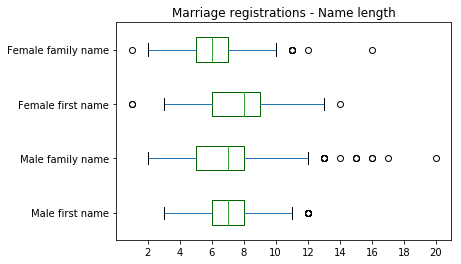
\includegraphics[scale=0.6]{figures/avg_name_length_boxplot.png}
		\label{fig:4.1}
	\end{center}
	
\end{figure}

When looking at the matches with a Levenshtein distance of 4 or 5, the distribution of the error over the names is also a good factor to take into consideration. An error of 4 or 5 in a single name could mean in some cases that more than half of the entire name of the candidate is different from the name of the target. Although the other three names do match completely (since the error is concentrated in a single name), the difference in that single name will render the match dubious. We will not take the type of name the error is in into account, i.e. we will treat an error of 3 in the first name of a male the same as an error of 3 in the last name of a female.  
We limit the matches we take from matches with a distance of 4 and 5 to those where the error is distributed over more than 1 name. For matches with a distance of 5, we will also ignore the matches which we have labeled `2,3` since these matches differ too much in two names. 

\section{Assessment of birth certificate matches}
Using the vectortree technique we will build sets of families. Using the name pairs and table \ref{tab:Ruleset} we can extend these families with all matches that are matched with a Levenshtein distance of 4 or 5, as described above. The next step is to assess the quality of the matching in the first step. 
Although the assessment of the quality of the matches can be done on any arbitrary matching, we will only assess the quality of the matches between the marriage certificates and the birth certificates here. The set of matches of the birth certificates to the marriage certificates of the parents are the most important set of matches to check for consistency, since these matches are directly related to the existence of a person: a person cannot exist if it is not born, although it is good to note that it is possible that birth certificates are missing or that a person migrated to the province of Zeeland before marrying. \\

There are four checks that can be carried out: 
\begin{itemize}
	\item Are the birth events after the marriage of the parents? \\
	Although children can be born before the parents are married, we do not consider these cases. Assuming that all birth events take place after the parents are married simplifies this check significantly. 
	\item Are there at least 10 months between two consecutive birth events within the same family?\\
	It is very unlikely that children will be born within 10 months from each other, since this is biologically almost an impossibility. 
	\item How long is the overall time span of birth events within the same family?\\
	If there is a gap of 20 years between two consecutive certificates, the likelihood that those certificate belong to the same family is smaller than when there is a gap of 5 years. 
	\item How long is the time span between the marriage of the parents and the birth certificate?
	The time span between the marriage and the birth events can not be greater than 25 years. Lowering this range might make this check more discriminative between families of parents and children with the same name, but it might also pose a problem when looking at large families. 
\end{itemize} 

In order to be accepted as a true match, the match must be compliant with all these four criteria.

 
